%"思考Python:像计算机科学家一样思考"LaTex源码
%Copyright (c) 2008 Allen B. Downey.
%中文翻译:2010 Walter Lewis (刘宇辉).

% Permission is granted to copy, distribute and/or modify this
% document under the terms of the GNU Free Documentation License,
% Version 1.1  or any later version published by the Free Software
% Foundation; with no Invariant Sections, no Front-Cover Texts,
% and no Back-Cover Texts.

% This distribution includes a file named fdl.tex that contains the text
% of the GNU Free Documentation License.  If it is missing, you can obtain
% it from www.gnu.org or by writing to the Free Software Foundation,
% Inc., 59 Temple Place - Suite 330, Boston, MA 02111-1307, USA.
%

\documentclass[10pt]{book}
\usepackage[width=5.5in,height=8.5in,
	hmarginratio=3:2,vmarginratio=1:1]{geometry} %指定了{h,v}marginratio,width和height被忽略了,可以不用指定(参考geometry.pdf, $texdoc geometry.pdf)。

%下面的这些包,你可能需要安装texlive-latex-extra(in Debian/Ubuntu)
\usepackage{pslatex}  %
\usepackage{url}
\usepackage{fancyhdr}
\usepackage{graphicx}
\usepackage{amsmath,amsthm,amssymb}
\usepackage{exercise}
\usepackage{makeidx}
\usepackage{setspace}
\usepackage{hevea}
\usepackage{upquote}
%这些是对中文的支持
\usepackage{xeCJK}
\usepackage{fontspec}
\setCJKmainfont{AR PL SungtiL GB:style=Regular}
\setmainfont{TeXGyrePagella:style=Regular}
\XeTeXlinebreaklocale "zh"
\XeTeXlinebreakskip=0pt plus 1pt minus 0.1pt

\title{思考Python}
\newcommand{\thetitle}{思考Python:像计算机科学家一样思考}
\newcommand{\theversion}{1.1.22}

%以下的这些风格被转换成html的css
\newstyle{a:link}{color:black;}
\newstyle{p+p}{margin-top:lem;margin-bottom:lem}
\newstyle{img}{border:opx}

%改变箭头(方向)
\setlinkstext
{\imgsrc[ALT="Previous"]{back.png}}
{\imgsrc[ALT="Previous"]{up.png}}
{\imgsrc[ALT="Previous"]{next.png}}

\makeindex

\begin{document}
\frontmatter
%LaTeXOnly

\input{latexonly}

\newtheorem{ex}{Exercise}[chapter]
\begin{latexonly}

\renewcommand{\blankpage}{\thispagestyle{empty} \quad \newpage}

%blankpage
%blankpage

%-half title----------------------------------------------
\thispagestyle{empty}
\begin{flushright}
\vspace*{2.0in}

\begin{spacing}{3}
{\huge 思考Python}\\
{\Large 像计算机科学家一样思考}
\end{spacing}

\vspace{0.25in}

Version \theversion

\vfill
\end{flushright}

%---------------------------
\blankpage
\blankpage

%---title page---------
\pagebreak
\thispagestyle{empty}

\begin{flushright}
\vspace*{2.0in}

\begin{spacing}{3}
{\huge 思考Python}\\
{\Large 像计算机科学家一样思考}
\end{spacing}

\vspace{0.25in}
Version \theversion

{\Large
	Allen Downey\\
}
{\Large 
	Walter Lewis\\
}



\vspace{0.5in}

{\Large Green Tea Press}\\
{\small Needham, Massachusetts}

\vfill
\end{flushright}

%---copyright------------------
\pagebreak
\thispagestyle{empty}

{\small
	Copyright \copyright ~2008 Allen Downey.

Printing history:

\begin{description}

\item[2002四月:] 第一版 {\em 像计算机科学家一样思考}.
\item[2007八月:] 大幅改动,把标题改为{\em 像(Python)程序员一样思考}.
\item[2008六月:] 大幅改动,把标题改为{\em 思考Python:像计算机科学家一样思考}.
\end{description}

\vspace{0.2in}

\begin{flushleft}  %左对齐,类似的有flushright,centre
Green Tea Press \\
9 Washburn Ave\\
Needham MA 02492
\end{flushleft}


Permission is granted to copy, distribute, and/or modify this document
under the terms of the GNU Free Documentation License, Version 1.1 or
any later version published by the Free Software Foundation; with no
Invariant Sections, no Front-Cover Texts, and with no Back-Cover Texts.

The GNU Free Documentation License is available from {\tt www.gnu.org}
or by writing to the Free Software Foundation, Inc., 59 Temple Place,
Suite 330, Boston, MA 02111-1307, USA.

The original form of this book is \LaTeX\ source code.  Compiling this
\LaTeX\ source has the effect of generating a device-independent
representation of a textbook, which can be converted to other formats
and printed.

The \LaTeX\ source for this book is available from
\url{http://www.thinkpython.com}
\vspace{0.2in}
}

\end{latexonly}


%htmlonly
\begin{htmlonly}

%Title page for html version

{\Large \thetitle}
\{\Large  Allen B.Downet}
\{\Large  翻译:Walter Lewis}

Version \theversion

\setcounter{chapter}{-1}
\end{htmlonly}

\chapter{前言}

\section{本书的奇怪历史}

1999年一月份的时候,我准备用Java教一门介绍性的编程课。在那之前,我已经
教了三次,而且每次我都很失望。这门课的挂课率非常之高,尽管对那些通过的学
生来说,整体的水平也是很低的。\\

我认为问题的根源之一是教科书。教科书太厚了,掺杂着大量不必要的Java细节
内容,并且没有足够高水平的引导去指导学生如何编程。学生们深陷“陷阱门“:他们起步很轻松,逐步的学习,突然,大约在第五章的某个位置,困难出现了。学生必须快速的学习大量的新内容。结果,我不得不把剩下的学期花在挑选一些片段来教学。\\

课程开始的前两周,我决定自力更生--自己编写书。我的目标是:
\begin{itemize}

\item 尽量简短.对学生来说,阅读十页比阅读无十页要好。

\item 注意词汇量。我尽量减少使用术语,而且在使用前必须先定义。

\item 逐步学习。为了避免陷阱门,我把最难的部分分解成一系列的小步骤。

\item 把重心放在编程,而不是编程语言。我采用最少的有用的Java语言的语法,
忽略其他的。
\end{itemize}

我需要一个书名,所以我就临时地把它叫做《像计算机科学家一样思考》\\

第一版很粗糙,但是很成功。学生们很乐意看它,并且能很好理解我在课堂上讲的难点,趣点和让他们实践的内容(这个最重要).\\

我用GNU自由文档许可证发布了这本书,读者们可以自由的复制,修改,发布这本书。 \\

\index{GNU Free Documentation License}
\index{Free Documentation License,GNU}

 接下来发生的事儿极其的有趣。Jeff Elkner,居住在弗尼亚的高中老师,改变了我的书,把它翻译成了Python。他给我寄了份他翻译的副本,于是乎我就有了一段不寻常的学习Python的经历--通过阅读我自己的书。\\

 Jeff和我随后修订了这本书,加入了Chris Meyers提供的一个案例学习。在2001年,我们共同发布了《像计算机科学家一样思考:Python编程》,当然同样是用GNU自由文档许可证。通过Gree Tea Press,我出版了这本书,并且开始在亚马逊和大学书店卖纸质书。Gree Tea Press出版的书可以从这儿获得\url{greenteapress.com}\\

 2003年,我开始在Olin College教书。第一次,我开始教Python。和教授Java的情况相反,学生们不再陷入泥潭,学到了更多,参与了很多有趣的项目,越学越带劲。\\

 在过去的五年里,我一直继续完善这本书,改正错误,提过某些例子的质量,加入一些其他的材料,特别是练习。在2008年,我开始重写这本书---同时,剑桥大学出版社的编辑联系到了我,他想出版本书的下一板。美妙的时刻!\\

 结构就出现了现在的这本书,不过有了一个简洁的名字《思考Python》。变化有:
 \begin{itemize}

 \item 在每一章末尾加了点调试的部分。这些部分提供了发现和避免bug的通用技巧,也对Python的陷阱提出了警告。

 \item 删除了最后几章关于列表和树实现的内容。虽然,我万分不舍,但是考虑到和本书余下的部分不协调,只能忍痛割爱。

 \item 增加了一些案例学习---提供了练习,答案和相关讨论的大例子。一些东西是基于Swampy,这是我为了教学而设计的Python程序。
 Swampy,代码实例和部分答案可以从这儿获得\url{thinkpython.com}.

 \item 扩展了关于程序构建计划和基本的设计模式的讨论。

 \item Python运用的更加地道。虽然这本书仍然是讨论编程的,而不是Python本身,但是现在我不得不承认这本书深受Python浸染。
 
 \end{itemize}

  我希望读者们可以享受这本书,也希望帮助你学习程序设计和像计算机科学家一样思考,哪怕是一丁丁点儿。\\

Allen B. Downey\\
Needham MA\\

Allen Downey 是Olin College 大学计算机科学与技术系的副教授。



\section*{声明}

首先,也是最重要的,我要感谢Jeff Elkner,是他把我的Java书翻译成了Python,也由此开启了这项“工程“,也把我领进了我最爱的编程语言大门。\\

我也要感谢Chris Meyers,他贡献了《像计算机科学家一样思考》的部分内容。\\

感谢FSF制定的GNU自由文档许可证,使我和Jeff 和Chris 的合作成为可能。\\

\index{GNU Free Documentation License}
\index{Free Documentation License,GNU}

我也要感谢所以使用以前版本的学生和所有的贡献者,他们提供了宝贵的更正和建议。\\

感谢我的妻子,Lisa为她在这本书上所花费的努力,还有Gree Tea Press,和其他的一切。

\section*{贡献者名单}

\index{贡献者}

More than 100 sharp-eyed and thoughtful readers have sent in
suggestions and corrections over the past few years.  Their
contributions, and enthusiasm for this project, have been a
huge help.

If you have a suggestion or correction, please send email to 
{\tt feedback@thinkpython.com}.  If I make a change based on your
feedback, I will add you to the contributor list
(unless you ask to be omitted).

If you include at least part of the sentence the
error appears in, that makes it easy for me to search.  Page and
section numbers are fine, too, but not quite as easy to work with.
Thanks!

\small

\begin{itemize}

\item Lloyd Hugh Allen sent in a correction to Section 8.4.

\item Yvon Boulianne sent in a correction of a semantic error in
Chapter 5.

\item Fred Bremmer submitted a correction in Section 2.1.

\item Jonah Cohen wrote the Perl scripts to convert the
LaTeX source for this book into beautiful HTML.

\item Michael Conlon sent in a grammar correction in Chapter 2
and an improvement in style in Chapter 1, and he initiated discussion
on the technical aspects of interpreters.

\item Benoit Girard sent in a
correction to a humorous mistake in Section 5.6.

\item Courtney Gleason and Katherine Smith wrote {\tt horsebet.py},
which was used as a case study in an earlier version of the book.  Their
program can now be found on the website.

\item Lee Harr submitted more corrections than we have room to list
here, and indeed he should be listed as one of the principal editors
of the text.

\item James Kaylin is a student using the text. He has submitted
numerous corrections.

\item David Kershaw fixed the broken {\tt catTwice} function in Section
3.10.

\item Eddie Lam has sent in numerous corrections to Chapters 
1, 2, and 3.
He also fixed the Makefile so that it creates an index the first time it is
run and helped us set up a versioning scheme.  

\item Man-Yong Lee sent in a correction to the example code in
Section 2.4.  

\item David Mayo pointed out that the word ``unconsciously"
in Chapter 1 needed
to be changed to ``subconsciously".

\item Chris McAloon sent in several corrections to Sections 3.9 and
3.10.

\item Matthew J. Moelter has been a long-time contributor who sent
in numerous corrections and suggestions to the book.  

\item Simon Dicon Montford reported a missing function definition and
several typos in Chapter 3.  He also found errors in the {\tt increment}
function in Chapter 13.

\item John Ouzts corrected the definition of ``return value"
in Chapter 3.

\item Kevin Parks sent in valuable comments and suggestions as to how
to improve the distribution of the book.

\item David Pool sent in a typo in the glossary of Chapter 1, as well
as kind words of encouragement.

\item Michael Schmitt sent in a correction to the chapter on files
and exceptions.

\item Robin Shaw pointed out an error in Section 13.1, where the
printTime function was used in an example without being defined.

\item Paul Sleigh found an error in Chapter 7 and a bug in Jonah Cohen's
Perl script that generates HTML from LaTeX.

\item Craig T. Snydal is testing the text in a course at Drew
University.  He has contributed several valuable suggestions and corrections.

\item Ian Thomas and his students are using the text in a programming
course.  They are the first ones to test the chapters in the latter half
of the book, and they have made numerous corrections and suggestions.

\item Keith Verheyden sent in a correction in Chapter 3.

\item Peter Winstanley let us know about a longstanding error in
our Latin in Chapter 3.

\item Chris Wrobel made corrections to the code in the chapter on
file I/O and exceptions. 

\item Moshe Zadka has made invaluable contributions to this project.
In addition to writing the first draft of the chapter on Dictionaries, he
provided continual guidance in the early stages of the book.

\item Christoph Zwerschke sent several corrections and
pedagogic suggestions, and explained the difference between {\em gleich}
and {\em selbe}.

\item James Mayer sent us a whole slew of spelling and
typographical errors, including two in the contributor list.

\item Hayden McAfee caught a potentially confusing inconsistency
between two examples.

\item Angel Arnal is part of an international team of translators
working on the Spanish version of the text.  He has also found several
errors in the English version.

\item Tauhidul Hoque and Lex Berezhny created the illustrations
in Chapter 1 and improved many of the other illustrations.

\item Dr. Michele Alzetta caught an error in Chapter 8 and sent
some interesting pedagogic comments and suggestions about Fibonacci
and Old Maid.

\item Andy Mitchell caught a typo in Chapter 1 and a broken example
in Chapter 2.

\item Kalin Harvey suggested a clarification in Chapter 7 and
caught some typos.

\item Christopher P. Smith caught several typos and helped us
update the book for Python 2.2.

\item David Hutchins caught a typo in the Foreword.

\item Gregor Lingl is teaching Python at a high school in Vienna,
Austria.  He is working on a German translation of the book,
and he caught a couple of bad errors in Chapter 5.

\item Julie Peters caught a typo in the Preface.

\item Florin Oprina sent in an improvement in {\tt makeTime},
a correction in {\tt printTime}, and a nice typo.

\item D.~J.~Webre suggested a clarification in Chapter 3.

\item Ken found a fistful of errors in Chapters 8, 9 and 11.

\item Ivo Wever caught a typo in Chapter 5 and suggested a clarification
in Chapter 3.

\item Curtis Yanko suggested a clarification in Chapter 2.

\item Ben Logan sent in a number of typos and problems with translating
the book into HTML.

\item Jason Armstrong saw the missing word in Chapter 2.

\item Louis Cordier noticed a spot in Chapter 16 where the code
didn't match the text.

\item Brian Cain suggested several clarifications in Chapters 2 and 3.

\item Rob Black sent in a passel of corrections, including some
changes for Python 2.2.

\item Jean-Philippe Rey at Ecole Centrale
Paris sent a number of patches, including some updates for Python 2.2
and other thoughtful improvements.

\item Jason Mader at George Washington University made a number
of useful suggestions and corrections.

\item Jan Gundtofte-Bruun reminded us that ``a error'' is an error.

\item Abel David and Alexis Dinno reminded us that the plural of
``matrix'' is ``matrices'', not ``matrixes''.  This error was in the
book for years, but two readers with the same initials reported it on
the same day.  Weird.

\item Charles Thayer encouraged us to get rid of the semi-colons
we had put at the ends of some statements and to clean up our
use of ``argument'' and ``parameter''.

\item Roger Sperberg pointed out a twisted piece of logic in Chapter 3.

\item Sam Bull pointed out a confusing paragraph in Chapter 2.

\item Andrew Cheung pointed out two instances of ``use before def.''

\item C. Corey Capel spotted the missing word in the Third Theorem
of Debugging and a typo in Chapter 4.

\item Alessandra helped clear up some Turtle confusion.

\item Wim Champagne found a brain-o in a dictionary example.

\item Douglas Wright pointed out a problem with floor division in
{\tt arc}.

\item Jared Spindor found some jetsam at the end of a sentence.

\item Lin Peiheng sent a number of very helpful suggestions.

\item Ray Hagtvedt sent in two errors and a not-quite-error.

\item Torsten H\"{u}bsch pointed out an inconsistency in Swampy.

\item Inga Petuhhov corrected an example in Chapter 14.

\item Arne Babenhauserheide sent several helpful corrections.

\item Mark E. Casida is is good at spotting repeated words.

\item Scott Tyler filled in a that was missing.  And then sent in
a heap of corrections.

\item Gordon Shephard sent in several corrections, all in separate
emails.

\item Andrew Turner {\tt spot}ted an error in Chapter 8.

\item Adam Hobart fixed a problem with floor division in {\tt arc}.

\item Daryl Hammond and Sarah Zimmerman pointed out that I served
up {\tt math.pi} too early.  And Zim spotted a typo.

\item George Sass found a bug in a Debugging section.

\item Brian Bingham suggested Exercise~\ref{exrotatepairs}.

\item Leah Engelbert-Fenton pointed out that I used {\tt tuple}
as a variable name, contrary to my own advice.  And then found
a bunch of typos and a ``use before def.''

\item Joe Funke spotted a typo.

\item Chao-chao Chen found an inconsistency in the Fibonacci example.

\item Jeff Paine knows the difference between space and spam.

\item Lubos Pintes sent in a typo.

\item Gregg Lind and Abigail Heithoff suggested Exercise~\ref{checksum}.

\item Max Hailperin has sent in a number of corrections and
  suggestions.  Max is one of the authors of the extraordinary {\em
    Concrete Abstractions}, which you might want to read when you are
  done with this book.

\item Chotipat Pornavalai found an error in an error message.

\item Stanislaw Antol sent a list of very helpful suggestions.

\item Eric Pashman sent a number of corrections for Chapters 4--11.

\item Miguel Azevedo found some typos.

\item Jianhua Liu sent in a long list of corrections.

\item Nick King found a missing word.

\item Martin Zuther sent a long list of suggestions.

\item Adam Zimmerman found an inconsistency in my instance
of an ``instance'' and several other errors.

\item Ratnakar Tiwari suggested a footnote explaining degenerate
triangles.

\item Anurag Goel suggested another solution for \verb"is_abecedarian"
and sent some additional corrections.  And he knows how to
spell Jane Austen.

\item Kelli Kratzer spotted one of the typos.

\item Mark Griffiths pointed out a confusing example in Chapter 3.

\item Roydan Ongie found an error in my Newton's method.

\item Patryk Wolowiec helped me with a problem in the HTML version.

\item Mark Chonofsky told me about a new keyword in Python 3.0.

\item Russell Coleman helped me with my geometry.

\item Wei Huang spotted several typographical errors.

\item Karen Barber spotted the the oldest typo in the book.

\item Nam Nguyen found a typo and pointed out that I used the Decorator
pattern but didn't mention it by name.

\item St\'{e}phane Morin sent in several corrections and suggestions.

\item Paul Stoop corrected a typo in \verb+uses_only+.

\item Eric Bronner pointed out a confusion in the discussion of the
order of operations.

\item Alexandros Gezerlis set a new standard for the number and
quality of suggestions he submitted.  We are deeply grateful!

% ENDCONTRIB

\end{itemize}


\normalsize
\clearemptydoublepage

\begin{latexonly}

\tableofcontents

\clearemptydoublepage

\end{latexonly}

\mainmatter

\chapter{编程的方式}

这本书的的目的是教会大家如何像计算机科学家一样思考。计算机科学用严谨的语言来表明思想,尤其是计算。像工程师,他们设计,把各个组件装配成系统并且在可选方案中评估出折中方案。像科学家,他们研究复杂系统的性能,做出假定并且测试假设。


\index{解决问题}

对一个计算机科学家来说最重要的是解决问题。解决问题意味着清晰明确的阐述问题,积极思考问题答案,并且清楚正确的表达答案的能力。实践证明:学习如何编程是一种很好的机会来练习解决问题的技巧。这也是为什么把这章叫做“编程的方式“。\\

一方面,你将学习编程,一个非常有用的技巧。另一方面你将会把编程作为一种科技。随着我们的深入学习,这点会渐渐明晰。

\section{Python编程语言}
\index{编程语言}
\index{语言!编程}

我们将要学习的编程语言是Python。Python仅是高级语言中的一种,你可能
也听说过其他的高级编程语言,比如C,C++,Perl,和Java。\\

也有一些低级语言,有时也被称为机器语言或者汇编语言。一般来说,计算机
只能执行用低级语言编写的程序。所以,用高级语言编写的程序在执行前必须
做相应的处理。这会花费一定的时间,同时这也是高级语言的“缺点“。\\

\index{移植性}
\index{高级语言}
\index{低级语言}
\index{语言!高级}
\index{语言!低级}

然而,高级语言的优点也是无限的。首先,用高级语言编程是一件非常容易的。
用高级语言编程通常花费的时间比较少,同时编写的程序简短,易读,易纠错
。第二,高级语言是可移植的,这意味着他们可以不加修改(或者修改很少)地运行在不同的平台上。低级语言编写的程序只能在一个机器上运行,如果想
要运行在另外一台机器上,必须得重写。\\

基于这些优点,几乎所有的程序都是用高级语言编写的。低级语言统称仅仅用
在一些专门的应用程序中。

\index{complie}
\index{interpret}

有两种程序把高级语言“处理”成低级语言:解释器和编译器。解释器读取源程序,解释执行,也就是按照程序表达的意思"做事"。解释器一次解释一点,或者说,一次读取一行,然后执行。\\

\beforefig
\centerline{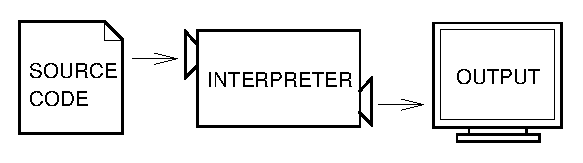
\includegraphics[height=0.77in]{figs/interpret.eps}}
\afterfig

\index{源码}
\index{目标}
\index{可执行代码}

编译器读取程序,完全转换之。在这种情况下,高级语言程序叫做源码,编译后的程序叫做目标代码或者叫可执行代码。一旦程序被编译,就可以直接执行,无须再编译。

\beforefig
\centerline{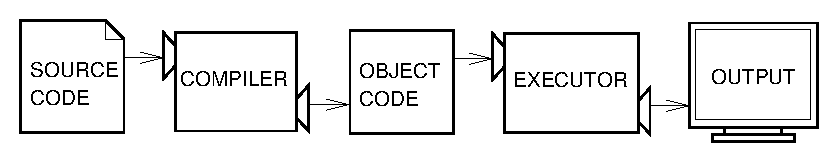
\includegraphics[height=0.77in]{figs/compile.eps}}
\afterfig

一般地,我们把python当作是解释型语言,因为用Python编写的程序是通过
解释器执行的。有两种使用解释器的方式:交互模式和脚本模式。在交互模式
下,你可以输入Python程序,然后解释器输出结果:

\index{交互模式}
\index{脚本模式}

\beforeverb
\begin{verbatim}    
>>>1 + 1
2
\end{verbatim} %直接输出以上两句,包括空白和断行
\afterverb

锯齿符,{\tt >>>},是提示符,解释器用它来表明自己已经准备好了,
如果你输入{\tt 1 + 1},解释器显示{\tt 2}。\\

\index{提示符}

另外地,我们可以把代码存储在一个文件里,使用解释器执行文件,此时这个
文件被称作脚本。习惯上,Python脚本的扩展名为{\tt .py}。

\index{脚本}

如果要执行Python脚本,我们必须提供给解释器脚本的文件名。在UNIX命令窗口,可以输入{\tt python dinsdale.py}。在其他开发环境中,会有些细节方面的差别。可以在Python官网上(\url{python.org})找到相应的指导。

\index{测试!交互模式}

在交互模式下工作很容易测试一小段代码,因为可以随时输入,并且立刻执行。但如果代码量较大,我们必须把代码存放在脚本里,这样方便我们以后修改执行。 

\section{什么是程序}

程序就是指令集合,这些指令说明了如何执行计算。计算可能是数学上的,例如解决等式组或者计算多项式的平方根。但是也可以是符号计算,比如搜索替换文件的文本或者(非常奇怪)编译一个程序。

\index{程序}

不同的语言有一些细节上的差异。但是他们有一些共有的指令:

\begin{description}

\item[输入:] 从键盘获取数据,文件,或者从其他设备。

\item[输出:] 在显示器上显示数据或者把数据输出到文件或其他设备。

\item[数学运算:] 做基本的数学操作像加法和乘法。

\item[条件执行:]检查条件,然后执行正确的语句。

\item[循环:]重复执行一些动作,通常有些变化。

\end{description}

信不信由你,就是这样。我们用过的任何一个软件,无论多么复杂,基本上都是由与这些相似的指令组成。所以,我们可以这么理解:编程就是把复杂庞大的任务分解为一系列的小任务,知道这些小任务简单到可以用这些基本的指令表示。

\index{算法}

这个有点模糊,但是当我们讲到算法的时候,我们再回过头来聊这个话题。

\section{什么是调试?}
\index{调试}
\index{臭虫}

有三种错误经常在程序中出现:语法错误,运行时错误和语义错误。为了能够快速的跟踪捕捉到他们,区分他们之间的诧异还是很有好处的。

\subsection{语法错误}
\index{语法错误}
\index{错误!语法}
\index{错误信息}

Python只能执行语法正确的程序;否则,解释器就会报错。语法指的是程序的结构和结构的规则。\index{syntax 语法}
比如,括号必须是成对出现,所以{\tt (1 + 2)}是合法的,但{\tt 8)}就是语法错误。

\index{parentheses!matching  括号!匹配}
\index{syntax 语法}
\index{cummings, e. e. 康明思}

在英语中,读者可以忍受大多数语法错误,这就是为什么我们玩味E. E康明思的诗歌,而没有提出任何错误信息的原因。Python不会这么仁慈。如果在你程序的某个地方出现了哪怕是一个语法错误,Python也会显示错误信息然后退出,你也不能再继续执行程序。在你初学编程的几周里,你很可能会花费大量的时间追踪,捕捉语法错误。一旦你有经验了,你犯的错误就更少,并且也能很快的发现他们。

\subsection{运行时错误}
\label{runtime 运行时}
\index{runtime error 运行时错误}
\index{error!runtime 错误!运行时}
\index{exception 异常}
\index{safe language 安全语言}
\index{language!safe 语言!安全}


第二中错误是运行时错误,之所以这么命名是因为从这种错误知道程序开始运行才会出现。这些错误也叫做异常,因为他们通常表明异常的事情发生了。\\

运行时错误在前几章的简短的代码中比较少见,因此你可能会有一段时间才会遇到。

\section{语义错误}
\index{semantics 语义}
\index{semantics errors 语义错误}
\index{error!semantic 错误!语义}
\index{error message 错误信息}

第三中错误是语义错误。如果有语义错误,程序会成功运行(即计算机不会产生任何的错误信息),但是它却没有做对!计算机做了另外的事。确切的说,计算机确实做了你告诉他的指令。

\subsection{试验性的调试}

你必须拥有的一条技能是调试。尽管在这个过程中,你可能很受伤,但,调试是编程中最具有挑战,最有意思,最能考验智力的一部分。\\

\index{experimental debugging 实验性的调试}
\index{debugging!experimental 调试!实验}

某种程度上,调试就像是侦探。你面对着很多线索,必须推断导致你看到的结果的过程和事件。\\

调试也像是一个科学实验。一旦你意识到错误的地方,改正她,再尝试。如果你的假想是正确的,你就可以预测出改变带来的结果,你也就离能够执行的程序更近一步了。如果你的猜想是错误的,你不得不提出一个新的。正如Sherlock Holmoes指出的,“当你移除了不可能的,留下来的无论是什么,也不论多么不可能,都是真理。(A. Conan Doyle, {\em The Sign of Four})\\

\index{Holems, Sherlock}
\index{Doyle, Arthur Conan}

对某些人来说,编程和调试是同时完成的。也就是,编程是不断调试,直到看到想要结果的过程。理念就是:你必须以一个能够工作的程序开始,然后做些小改动,随着进度不断调试他们,这样就总是有一个可工作的程序。\\

比如:Linux是一个包含成千上万行代码的操作系统,但它也是从一个Linux Torvalds用来研究Intel 80386芯片的小程序开始的。按照Larry Greenfield的说法,“Linus的早期项目就是一个在打印AAAA和BBBB之间切换的程序。“({\em The Linux Users' Guide} Beta Version 1)。

\index{Linux}

接下来的章节将介绍更多的调试建议还有其他的编程经验。

\section{正式语言和自然语言}
\index{formal language 正式语言}
\index{natural language 自然语言}
\index{language!formal 语言!正式}
\index{language!natural 语言!自然}

自然语言是人们日常说的语言,比如英语,西班牙语和法语。他们不是人民设计的(尽管人们努力的强加一些规则);他们是自然发展的。\\

正式语言是人们为了特别的应用而设计的语言。比如,数学家使用的符号就是一门正式语言,它很擅长揭示数字和符号之间的联系。化学家用正式语言代表分子的化学结构。最重要的是:

\begin{quote}
{编程语言是正式语言,是被设计来表达计算的。}
\end{quote}

正式语言倾向于有严谨的语法规则。比如,$3 + 3 = 6$是语法争取的数学语句。但是$3 += 3 \mbox{\$} 6$ 不是。$H_2O$是语法正确的化学分子式,但$_2Zz$ 不是。\\

语法规则涉及到两个方面:标记和结构。标记是语言的最基本元素,比如字,数字和化学元素。$3 += 3 \mbox{\$} 6$的一个问题是$\$$不是一个合法的数学标记(至少据我所知)。相似的,$_2Zz$不合法是因为没有元素的缩写是$Zz$。

\index{token 标记}
\index{structure 结构}

第二种语法错误涉及到语句的结构,也就是,标记被安排的方式。语句$3 + = 3 \mbox{\$} 6$是非法的因为尽管$+$和$=$是合法的标记,但我们不能把两个相连。同样的,在化学分子式中,下标必须在元素之后,不是前面。

\begin{ex}
写一个结构正确的英语句子,同时标记也必须合法。然后写一个结构不合理但是标记合法的句子。
\end{ex}

当阅读一个英文句子或者正式语言的一个语句,必须明确句子的结构(尽管对于自然语言来说,这个是潜意识的)。这个过程叫做句法分析。

\index{parse 句法分析}

比如,当你听到一个句子,“一便士硬币掉了”,你理解“一便士硬币”是主语,“掉了”是谓语。一旦你分析了这个句子,你就明确句子的意思。假如你知道一个便士是什么,并且什么是掉了,你就会明白这个句子的一般含意。\\

尽管正式语言和自然语言有很多共同点---标记,结构,语法和语义---也存在一些不同点:

\index{ambiguity 二义性}
\index{redundancy 冗余性}
\index{literalness 无修饰性}

\begin{description}

\item[二义性:]自然语言充满了二义性(模糊性),人们利用上下文来区分。正式语言被设计成近乎没有二义性,这也意味着每个语句都有明确的意思,无论上下文。

\item[冗余性:]为了弥补二义性和减少误解,自然语言设置了很多冗余。因此自然语言是冗长的。自然语言更简短,精确。

\item[无修饰性:]自然语言充满了习语和隐喻。如果我说“一便士硬币掉了”,也许根本没有便士也没有东西掉了\footnote{这个习语意思是某人困惑之后恍然大悟。}。正式语言表达了是精确的意思。

\end{description}

成长过程中,说自然语言的人---每个人---通常在调整自己适应正式语言的过程中都会经历痛苦。某种程度上,正式语言和自然语言之间的区别就像诗歌和散文\footnote{译者:这里的散文不是诗化的散文,像余光中老前辈开启的诗化散文}之间的区别,甚至更多:

\index{poetry 诗歌}
\index{prose 散文}

\begin{description}

\item[诗歌:]单词的运用既是为了语义的需要,也是为了音韵的需要,整首诗创造了一种情感共鸣。二义性不仅很常见,而且常常是故意安排的。

\item[散文:]单词的字面意思更加重要,结构也表达了更多的意思。散文比诗歌更容易分析,但是仍然具有二义性。

\item[程序:]计算机程序是无二义性。可以通过分析标记和结构完全理解。


\end{description}

这里给些读程序时候的一些建议(包括其他正式语言).第一,记住正式语言是比自然语言要晦涩的,所以要花长时间阅读。其次,结构也是非常重要的,所以,从头到位,从左到右阅读通常不是一个好的办法,可以学习在大脑中分析程序,识别标记的意思,然后解释结构。最后,细节也很重要。一些拼写和标点上细小的错误(在自然语言中可以忽略的),有时会在正式语言中掀起大浪。

\section{第一个程序}
\label{hello}
\index{Hello, World}

通常,学习新语言的第一个程序就是"hello world", 应为所做的就是显示单词,"Hello , World!".在Python中,看起来是:

\beforeverb
\begin{verbatim}
print 'Hello, World!'
\end{verbatim}
\afterverb

这是一个print语句的例子\footnote{在Python3.0中,{\tt print}是一个函数,不是一个语句了,所以语法是{\tt print("Hello, World!")}。我们不久就要接触到函数了!  译注:在本书翻译时python 2.7 和python3.1已经发布,python 3.2的release 版也即将发布},没有真正在纸上打印东西。它在显示器上显示了一个值。在这种情况下,结果是单词

\index{Python 3.0}

\beforeverb
\begin{verbatim}
Hello, World!
\end{verbatim}
\afterverb

程序中的引号标志了要被显示的文本的开始和结束,他们不会出现在结果中。

\index{quotation mark 引号}
\index{print statement print 语句}
\index{statement!print 语句!打印}

一些人通过"Hello, World!"程序的简洁程度来判断编程语言的好坏。按照这个标准,Python确实非常好!


\section{调试}
\index{debugging 调试}

坐在电脑前面看这本书是个不错的方法,你可以随时尝试书中的例子。你可以在
交互模式下运行大多数的程序,但是如果你把代码放在一个脚本里,也是很容易尝试改变一些内容的。\footnote{译者注:我的理解是,可以很方便的
改动某些变量或者语句,然后执行}\\

无论何时,尝试一个新的特点的时候,你应该故意的犯些错误。比如,在"Hello, World!"程序中,如果忽略了双引号其中之一,会发生什么?如果把两个引号都忽略了,又会怎样?如果拼错了{\tt print}了呢?\\

\index{error message 错误信息}

这种实验能够有效的帮助你记住你看的内容,同时也对调试有好处,因为你知道了错误信息的意思了。现在故意的犯错误总比以后猝不及防的犯错误要好的多。\\

编程,特别是调试,有时带来很强的情绪。你在一个困难的bug里苦苦挣扎,你可能变得怒不可遏,苦恼不堪,甚至羞愧不已。\\

有证据表明,人们很容易把电脑当成人来对待\footnote{参看Reeves和Nass,{\it The Media Equation:How People Treat Computers, Television, and New Media Like Real People and Places}.}.当电脑工作正常,我们把它们当作是队友,当电脑不给力时,我们把它们当成粗鲁顽固的人。\\

\index{debugging!emotional response 调试!情绪反应}
\index{emotional debugging 情绪调试}

为这些反应作准备也许会帮助你合理的处理。一个方法是把电脑当作一个员工,他既拥有一定力量,比如速度和精度,也会有特别的缺点,比如缺少默契,没有能力理解大的图片。\\

你的工作就是做一个好的经理:发掘有效的方法扬长补短。并且寻找方法利用你的情绪来投入到解决问题中,不要让你的(不良)反应干扰你工作的能力.\\

学习调试是令人沮丧的,但是一种宝贵的技巧,在编程的其他领域也是大有裨益的。在每章的末尾,都有一个调试段落,像这个一样,是我调试经验的总结。我希望他们对你有益!

\section{术语表}
\begin{description}

\item[problem solving 问题解决:]表述问题,发现解,表达解的过程。

\item[high-level language 高级语言:]像Python一样的程序设计语言,被设计让人们易读易写程序。

\item[low-level language 低级语言:]设计让计算机容易执行的程序设计语言;也叫做“机器语言”或者“汇编语言”。

\item[portability 可移植性:]程序可以在一台或多台电脑执行的属性。

\item[interpret 解释:]逐行逐行解释执行用高级语言编写的程序。

\item[compile 编译:]把用高级语言编写的程序转换成低级语言。
\index{compile 编译}

\item[source code 源码:]未编译的高级语言编写的程序。

\item[object code 目标代码:] 编译器转换程序后的输出。
\index{object code 目标代码}

\item[executable 可执行代码:] 目标代码的别名,可以被执行。
\item{executable 可执行代码}
\item[prompt 提示符:] 解释器显示的字符,表明做好准备让用户输入。
\index{prompt 提示符}

\item[script 脚本:]存储在文件中的程序。
\index{script 脚本}

\item[interactive mode 交互模式:] 一种通过输入命令和表达式的使用python解释器的方式。
\index{interactive mode 交互模式}

\item[script mode 脚本模式:] 一种使用Python解释器的方式,Python解释器读取脚本中的语句执行。
\index{script mode 脚本模式}

\item[program 程序:]指明计算的指令集合。
\index{program 程序}


\item[algorithm 算法] 求解一类问题的通用过程。
\index{algorithm}

\item[bug:] 程序的错误。
\index{bug}

\item[debugging 调试:]发现,去除程序错误的过程。
\index{debugging 调试}

\item[syntax 语法] 程序的结构。
\index{syntax 语法} 

\item[syntax error 语法错误:]使程序不能正确解析的错误。
\index{syntax error}


\item[exception 异常:]程序在运行时发现的错误。
\index{exception 异常}

\item[semantics  语义:]程序的含意。
\index{semantics 语义}

\item[semantics error 语义错误:] 程序中的错误,使计算机执行另外的程序。
\index{semantics error 语义错误}

\item[natural language 自然语言:]人们日常交流用的语言,自然发展的。
\index{natural language 自然语言}

\item[formal language 正式语言:]人民为了某种特殊目的设计的语言,比如,代表数学思想或者计算机程序,所有的程序设计语言都是正式语言。
\index{formal language 正式语言}

\item[token 标记:]程序语法结构的最基本元素,类似于自然语言的单词。
\index{token 标记}

\item[parse 句法分析:]检查程序,分析语法结构。
\index{parse 句法分析}

\item[print statement print 语句:]一条指示Python解释器显示一个值的指令。
\index{print statement print 语句}

\index{statement!print 语句!打印}

\end{description}

\section{练习}

\begin{ex}
打开浏览器浏览Python官网\url{python.org}.这个页面包含了Python的一些信息,还有和Python相关的连接。你可以查看Python官方文档。\\

比如,在搜索框里输入{\tt print},第一个链接就是{\tt print}语句的文档。此时,并不是所有的信息对你都有意义,但是知道它们在哪里总是有好处的。

\index{documentation 文档}
\index{python.org}
\end{ex}

\begin{ex}
启动Python的解释器,输入{\tt help()}启动在线帮助工具。或者你也可以输入\verb"help('print')" 获得关于{\tt print}语句的信息。\\

如果没有成功,你或许需要安装额外的Python官方文档,或者设置环境变量。这个依赖于你使用的操作系统和Python解释器版本。

\index{help utility 帮助工具}
\end{ex}


\begin{ex}
打开Python解释器,我们暂且把它作为计算器。关于数学操作的语法,Python和标准的数学符号很相似。比如,符号{\tt +},{\tt -} 和{\tt /}表示加减,除。乘法的符号是{\tt *}。\\

如果43分钟30秒,跑了10公里,每英里花费的时间是多少?你的平均速度是多少英里每小时?(Hint:一英里等于1.61公里)。

\index{caculator 计算器}
\index{running pace 跑步速度}
\end{ex}

























\end{document}
